\chapter{Teoría de las curvas elípticas}

\section{Introducción y motivación}
Los sistemas criptográficos que usan las curvas elípticas dependen de la aritmética de los puntos de la curva. Como hemos mencionado anteriormente en el capítulo~\ref{chap:Campos_finitos}, la eficiencia de estos esquemas basados en curvas elípticas depende directamente de la velocidad de los algoritmos de aritmética de curva, que a su vez recaen en las operaciones sobre el campo (suma, multiplicación, inversión)...

La figura~\ref{fig:ECDSA_esquema} muestra las bases necesarias para entender e implementar un protocolo como el algoritmo de firma digital de curva elíptica (ECDSA). La aritmética de curvas no solo se construye sobre las operaciones en el campo subyacente, sino que en algunos casos también requiere aritmética de grandes enteros y operaciones modulares. ECDSA emplea una función hash y ciertas operaciones modulares, pero los pasos más costosos desde el punto de vista computacional son las propias operaciones en la curva.
\begin{figure}[H]
    \centering
    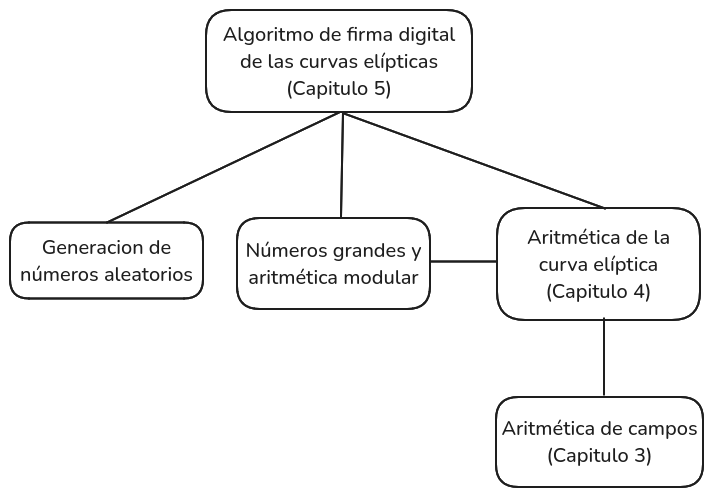
\includegraphics[width=0.8\textwidth]{imagenes/ECDSA_esquema.png}
    \caption{Esquema del Algoritmo de firma digital de las curvas elípticas (ECDSA)}
    \label{fig:ECDSA_esquema}
\end{figure}
%need to update this
La sección~\ref{sec:historia_curvas_elipticas} ofrece una introducción a las curvas elípticas donde se presentan las operaciones de grupo de suma y duplicado para los puntos de la curva, junto con su estructura fundamental y otras propiedades básicas. La sección~3.2 expone las representaciones en coordenadas proyectivas (y los algoritmos asociados de suma y duplicado), de especial interés cuando la inversión en el campo es más cara que la multiplicación. La sección~3.3 discute estrategias para la multiplicación de puntos.

Los métodos de las secciones~3.4, 3.5 y 3.6 están relacionados en que todos ellos explotan endomorfismos de la curva para reducir el coste del duplicado en la multiplicación de puntos. La sección~3.4 trata las curvas de Koblitz especiales, que permiten sustituir el duplicado de punto sobre \(\mathbb{F}_2\) por operaciones de cuadrado en el campo, mucho más baratas. La sección~3.5 examina una clase más amplia de curvas elípticas que admiten endomorfismos usados eficientemente para disminuir el número de duplicaciones. Las estrategias de la sección~3.6, para curvas sobre campos binarios, reemplazan la mayoría de los duplicados por una operación de “halving” de punto, potencialmente más rápida. La sección~3.7 recoge comparaciones de conteo de operaciones para métodos seleccionados de multiplicación de puntos. Finalmente, la sección~3.8 concluye con notas del capítulo y referencias.


\subsection{Historia}\label{sec:historia_curvas_elipticas}
Las curvas elípticas nacen del problema de calcular la longitud de arco de una elipse, que John Wallis abordó en 1655, y se articulan primero como integrales elípticas gracias a los pioneros Giulio Fagnano y Leonhard Euler en la primera mitad del siglo XVIII. En 1786, Adrien-Marie Legendre sistematiza estas integrales en tres “tipos” y sienta las bases de las funciones elípticas. A finales de la década de 1820, Niels Abel y Carl Jacobi invierten estas integrales, dando lugar a la teoría clásica de funciones elípticas. A mediados del siglo XIX, Karl Weierstrass y Bernhard Riemann las conectan con la estructura algebraico‐geométrica de curvas de género uno (tóricas complejas). Finalmente, en el siglo XX, Louis Mordell y André Weil desarrollan la teoría aritmética de puntos racionales, abriendo paso a la geometría algebraica moderna.

\section{Definición de una curva elíptica}\label{sec:definicion_curvas_elipticas}
\begin{definicion}[Curva elíptica sobre un cuerpo]\label{def:definicion_curvas_elipticas}
Sea $K$ un cuerpo. Una \emph{curva elíptica} $E$ sobre $K$ es un modelo de Weierstrass generalizado de la forma
\begin{equation}\label{eq:weierstrass_generalizada}
  E:\quad y^2 + a_1\,x\,y \;+\; a_3\,y \;=\; x^3 + a_2\,x^2 + a_4\,x + a_6,
\end{equation}
donde
\[
a_1,\;a_2,\;a_3,\;a_4,\;a_6 \;\in\; K,
\]
sujeto a la condición de no singularidad que expresaremos a continuación.

\medskip

\noindent\textbf{Invariantes auxiliares.} Definimos los siguientes invariantes:
\[
\begin{aligned}
  d_2 &= a_1^2 + 4a_2, &\quad
  d_4 &= 2a_4 + a_1 a_3,\\
  d_6 &= a_3^2 + 4a_6, &\quad
  d_8 &= a_1^2 a_6 + 4a_2 a_6 - a_1 a_3 a_4 + a_2 a_3^2 - a_4^2.
\end{aligned}
\]

\medskip

\noindent\textbf{Discriminante.} El discriminante de la ecuación \eqref{eq:weierstrass_generalizada} se define por
\[
  \Delta \;=\;-\,d_2^2\,d_8 \;-\; 8\,d_4^3 \;-\; 27\,d_6^2 \;+\; 9\,d_2\,d_4\,d_6.
\]
Con la condición necesaria $\Delta \;\neq\; 0$.

\medskip

\noindent\textbf{Punto en el infinito y conjunto de puntos racionales.}  
Denotamos por $\infty$ el único punto en el infinito (punto de Weierstrass) que completa la curva para obtener un cuerpo de funciones de género 1. Para cualquier extensión de cuerpos $L/K$, el conjunto de puntos de $E$ con coordenadas en $L$ viene dado por
\[
  E(L) \;=\; \bigl\{(x,y)\in L^2 : y^2 + a_1\,x\,y + a_3\,y - x^3 - a_2\,x^2 - a_4\,x - a_6 = 0 \bigr\}
  \;\cup\;\{\infty\}.
\]
\end{definicion}


\subsection{Comentarios sobre la definición~\ref{def:definicion_curvas_elipticas}}
\begin{enumerate}
  \item La ecuación \eqref{eq:weierstrass_generalizada} se conoce como la \emph{ecuación de Weierstrass}.
  \item Decimos que \(E\) está \emph{definida sobre} \(K\) porque los coeficientes \(a_i\) pertenecen a \(K\). A menudo escribimos \(E/K\) y diremos que \(K\) es un \emph{cuerpo base}.
  \item La condición \(\Delta\neq0\) garantiza que la curva es \emph{suave}, es decir, no tiene singularidades (no hay puntos con dos tangentes distintas). Esto esencialmente viene dado por puntos que anulan las derivadas paricales de la siguiente función de una curva elíptica:
  \[
    f(x,y) = y^2 +a_1xy + a_3y -x^3 - a_2x^2 - a_4x - a_6
  \]
  Se puede encontrar un ejemplo donde \(\Delta\neq0\) en la figura ~\ref{fig:elliptic_curve_singular_example}.
  \item El punto \(\infty\) es el único punto de la "línea en el infinito" que satisface la forma proyectiva de la ecuación de Weierstrass.
  \item Los \emph{puntos \(L\)-racionales} de \(E\) son aquellos cuyos pares \((x,y)\) pertenecen al cuerpo \(L\). Siempre incluimos \(\infty\).
\end{enumerate}

\begin{figure}[H]
    \centering
    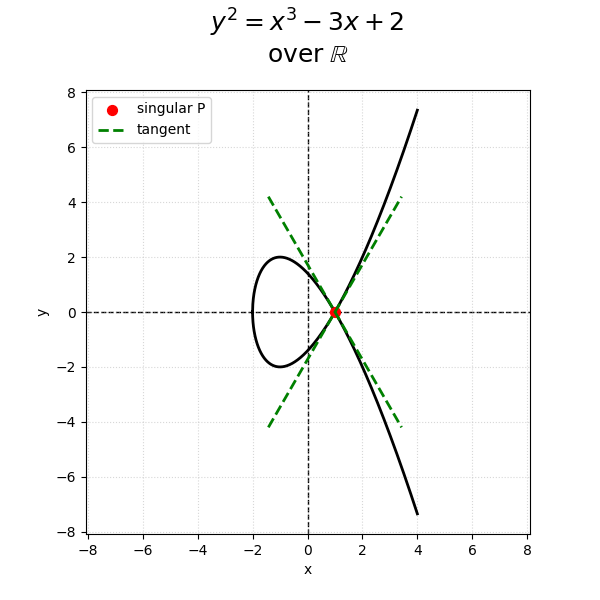
\includegraphics[width=0.8\textwidth]{imagenes/elliptic_curve_singular_example.png}
    \caption{Ejemplo de una curva elíptica con un punto singular, es decir, \(\Delta\neq0\)}
    \label{fig:elliptic_curve_singular_example}
\end{figure}

\begin{ejemplo}
Consideremos dos curvas elípticas sobre \(\mathbb{R}\):
\[
  E_1: \;y^2 = x^3 - 12x - 5,
  \qquad
  E_2: \;y^2 = x^3 + 3x + 15.
\]
Las gráficas de los conjuntos \(E_1(\mathbb{R})\setminus\{\infty\}\) y
\(E_2(\mathbb{R})\setminus\{\infty\}\) se muestran en la figura~\ref{fig:curvas_reales}.
\end{ejemplo}

\begin{figure}[H]
  \centering
  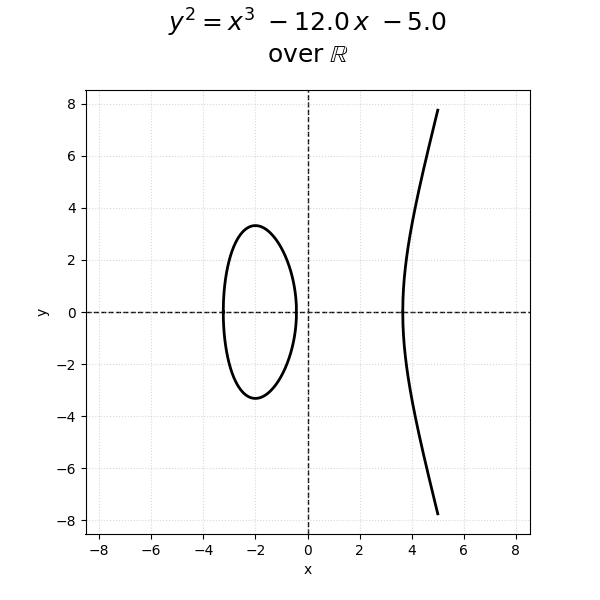
\includegraphics[width=0.48\textwidth]{imagenes/elliptic_curve2D_example.png}
  \hfill
  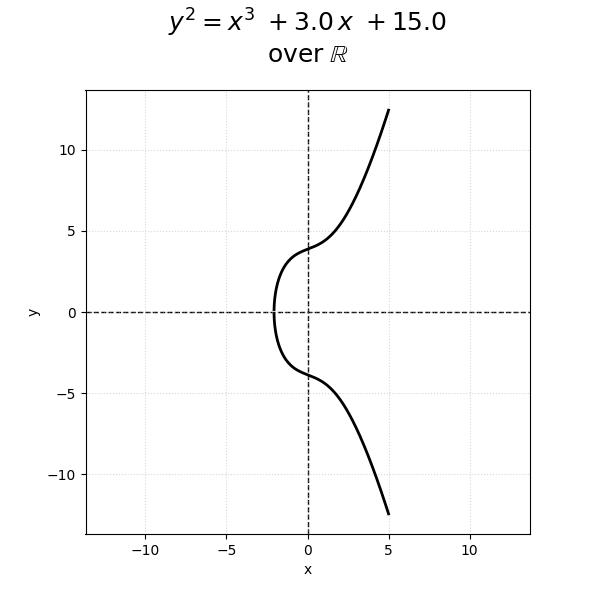
\includegraphics[width=0.48\textwidth]{imagenes/elliptic_curve2D_example2.png}
  \caption{Curvas \(E_1\) y \(E_2\) sobre \(\mathbb{R}\), con sus respectivos puntos (excepto \(\infty\)).}
  \label{fig:curvas_reales}
\end{figure}

\subsection{Ecuaciones simplificadas de Weierstrass}\label{sec:simplificaciones_weierstrass_curvas_elipticas}

\begin{definicion}
Sean dos curvas elípticas $E_1$ y $E_2$ definidas sobre un cuerpo $K$, dadas por las ecuaciones de Weierstrass

\[
\begin{aligned}
E_1:\; & y^2 + a_1 x y + a_3 y = x^3 + a_2 x^2 + a_4 x + a_6,\\
E_2:\; & y^2 + a_1 x y + a_3 y = x^3 + a_2 x^2 + a_4 x + a_6,
\end{aligned}
\]

se dice que $E_1$ y $E_2$ son \emph{isomorfas} sobre $K$ si existen $u,r,s,t\in K$, $u\neq0$, tales que el cambio de variables

\begin{equation}\label{eq:cambio_admisible}
(x,y)\longmapsto\bigl(u^2x + r,\;u^3y + u^2s,\;x + t\bigr)
\end{equation}

transforma la ecuación de $E_1$ en la de $E_2$. A dicho cambio se le llama \emph{admisible}.
\end{definicion}

\subsubsection*{1. Característica $\neq2,3$}

Si $\operatorname{char}(K)\neq2,3$, el cambio de variables admisible

\[
(x,y)\longmapsto\Bigl(x - \frac{3a_1^2 - 12a_2}{36},\;y - \frac{3a_1x}{216} - \frac{a_1^3 + 4a_1a_2 - 12a_3}{24}\Bigr)
\]

lleva
\[
y^2 + a_1xy + a_3y = x^3 + a_2x^2 + a_4x + a_6
\]
a la forma simplificada

\begin{equation}\label{eq:weierstrass_simple}
y^2 = x^3 + a x + b,
\end{equation}

donde $a,b\in K$. El discriminante de esta curva es

\[
\Delta = -16\bigl(4a^3 + 27b^2\bigr)\neq0.
\]

\paragraph{Razón algebraica de la simplificación}
Los cambios de variable implementan los pasos de "completar cuadrados" y "completar cubos" para eliminar los \emph{términos cruzados} (aquellos que mezclan $x$ e $y$ o que no son puramente $y^2$ o $x^3$) en la ecuación general:

\begin{itemize}
  \item Para suprimir $a_1xy + a_3y$, completamos el cuadrado en $y^2 + a_1xy + a_3y$ mediante
    \[
      y = y' - \frac{a_1}{2}\,x - \frac{a_3}{2},
    \]
    que requiere $\tfrac12\in K$ (por tanto $2\neq0$).
  \item Para eliminar el término $a_2x^2$ de la parte derecha, completamos el cubo en
    \[
      x^3 + a_2x^2 + \cdots
    \]
    aplicando
    \[
      x = x' + \frac{a_2}{3},
    \]
    que exige $\tfrac13\in K$ (por tanto $3\neq0$).
\end{itemize}

\paragraph{Ejemplo detallado:}
Sea $K=\mathbb{Q}$ y la curva
$$
y^2 + 6xy + 2y = x^3 + 9x^2 + 5x + 1.
$$

\textbf{Paso 1: Eliminación de $xy$, con}
$$
y = y' - 3x - 1.
$$
Sustituyendo en el lado izquierdo obtenemos:
$$
\begin{aligned}
\text{LHS} &= (y' - 3x - 1)^2 + 6x(y' - 3x - 1) + 2(y' - 3x - 1)\\
&= y'^2 -6xy' -2y' +9x^2 +6x +1\\
&\quad +6xy' -18x^2 -6x +2y' -6x -2\\
&= y'^2 -9x^2 -6x -1.
\end{aligned}
$$
Por tanto, la ecuación se convierte en
$$
y'^2 -9x^2 -6x -1 = x^3 +9x^2 +5x +1.
$$
Reordenamos:
$$
y'^2 = x^3 + (9+9)x^2 + (5+6)x + (1+1) = x^3 + 18x^2 +11x +2.
$$
Aquí $a_2' = 18$.

\textbf{Paso 2: Eliminación de $x^2$, con}
$$
x = x' + \frac{a_2'}{3} = x' + 6.
$$
Sustituyendo en el lado derecho y expandiendo:
$$
\begin{aligned}
x^3 + 18x^2 + 11x + 2 &= (x'+6)^3 + 18(x'+6)^2 + 11(x'+6) + 2\\
&= x'^3 + 18x'^2 + 108x' +216 \\ 
&\quad +18(x'^2+12x'+36) +11x' +66 +2\\
&= x'^3 + (18+18)x'^2 + (108+216+11)x' + (216+648+68)\\
&= x'^3 + 36x'^2 + 335x' + 932.
\end{aligned}
$$
Finalmente, tras restar el término $36x'^2$, obtenemos
$$
y'^2 = x'^3 + 335x' + 932,
$$
que ya está libre de $x'^2$.

\subsubsection*{2. Característica $2$}

En $\operatorname{char}(K)=2$ hay dos casos:

\paragraph*{2.1. Caso $\boldsymbol{a_1\neq0}$ (no supersingular)}  
El cambio
\[
(x,y)\longmapsto\Bigl(\tfrac{a_1^2\,x + a_3}{a_1},\;\tfrac{a_3^2\,y + a_1^2a_4 + a_3^2}{a_1^2}\Bigr)
\]
simplifica la ecuación general a
\begin{equation}\label{eq:f2m_nonsupersingular}
y^2 + xy = x^3 + A x^2 + B,
\end{equation}
con $A,B\in K$. Su discriminante es $\Delta = B\neq0$.

\paragraph*{2.2. Caso $\boldsymbol{a_1=0}$ (supersingular)}  
El cambio
\[
(x,y)\longmapsto(x + a_2,\;y)
\]
transforma la curva a
\begin{equation}\label{eq:f2m_supersingular}
y^2 + C\,y = x^3 + A x + B,
\end{equation}
donde $A,B,C\in K$. Su discriminante es $\Delta = C^4\neq0$.

\subsubsection*{3. Característica $3$}

En $\operatorname{char}(K)=3$ también hay dos casos:

\paragraph*{3.1. Caso $\boldsymbol{a_1^2 \neq -a_2}$ (no supersingular)}  
Definimos
\[
d_2 = a_1^2 + a_2,\qquad d_4 = a_4 - a_1a_3,
\]
y aplicamos el cambio
\[
(x,y)\longmapsto\Bigl(x + \tfrac{d_4}{d_2},\;y + a_1x + \tfrac{a_1\,d_4}{d_2} + a_3\Bigr).
\]
La ecuación resultante es
\begin{equation}\label{eq:f3_nonsupersingular}
y^2 = x^3 + A x^2 + B,
\end{equation}
con $A,B\in K$, y discriminante $\Delta = -A^3B\neq0$.

\paragraph*{3.2. Caso $\boldsymbol{a_1^2 = -a_2}$ (supersingular)}  
El sencillo cambio
\[
(x,y)\longmapsto(x,\;y + a_1x + a_3)
\]
conduce a la forma
\begin{equation}\label{eq:f3_supersingular}
y^2 = x^3 + A x + B,
\end{equation}
con $A,B\in K$ y discriminante $\Delta = -A^3\neq0$.

\subsubsection*{Interpretación y uso de las formas simplificadas}

La razón de distinguir tres familias de ecuaciones simplificadas responde a la imposibilidad de dividir por \(2\) o \(3\) cuando \(\mathrm{char}(K)\) es \(2\) o \(3\), lo que impide completar cuadrados y cubos para despejar los términos cruzados. Cada forma reducida se adapta a:
\begin{itemize}
  \item \textbf{Característica \(\neq2,3\) (ecuación corta de Weierstrass)}  
    \[
      y^2 = x^3 + ax + b.
    \]
    Es la forma \emph{short} más habitual en criptografía de curva elíptica sobre primos grandes, ya que minimiza el número de parámetros y simplifica las fórmulas de suma y duplicación~\cite{SilvermanAEC}. Todas las curvas estándar de NIST y SECG usan este modelo~\cite{NIST-SP-800-186}.
  \item \textbf{Característica \(2\) (campos binarios)}  
    \begin{align*}
      y^2 + x y &= x^3 + A x^2 + B
      &&\text{(no supersingular)},\\
      y^2 + C y &= x^3 + A x + B
      &&\text{(supersingular)}.
    \end{align*}
    En hardware ligero y tarjetas inteligentes, trabajar en \(\mathbb{F}_{2^m}\) sólo requiere desplazamientos y XOR, sin multiplicaciones completas de enteros~\cite{KoblitzBinary}. Las curvas no supersingulares se eligen para evitar vulnerabilidades a ataques basados en endomorfismos especiales.
  \item \textbf{Característica \(3\)}  
    \[
      y^2 = x^3 + A x^2 + B
      \quad\text{o}\quad
      y^2 = x^3 + A x + B,
    \]
    con distinción similar entre casos \emph{supersingular} y \emph{ordinarios}~\cite{SilvermanAEC}. Aunque menos comunes en criptografía práctica, estas curvas sirven en estudios teóricos y en construcciones avanzadas de pares bilineales.
\end{itemize}

\paragraph{Curvas ordinarias vs.\ supersingulares}  
La condición de \emph{supersingularidad} (discriminante especial, ver cada caso) refleja que el grupo de puntos de la curva tiene un anillo de endomorfismos más grande. Si bien ciertas construcciones pairing‐based usan curvas supersingulares (por sus endomorfismos explícitos), para ECC estándar se prefieren curvas \emph{ordinarias} (no supersingulares) para evitar ataques que explotan ese extra de simetría~\cite{Waterhouse1969}.  

\subsection{Ley de Grupo}\label{sec:ley_de_grupo}
Sea \(E\) una curva elíptica definida sobre un cuerpo \(K\). El conjunto de puntos \(E(K)\), junto con un elemento especial \(\O\) (punto en el infinito), adquiere una estructura de grupo abeliano mediante la llamada \emph{regla de la cuerda y la tangente}, basado en dos construcciones geométricas distintas, según si sumamos dos puntos distintos o duplicamos un mismo punto.

\subsubsection*{1. Suma de puntos distintos (\(P \neq Q\))}

\begin{enumerate}
  \item {\bf Geometría:} Dado \(P=(x_1,y_1)\) y \(Q=(x_2,y_2)\) con \(P\neq Q\), trazamos la \emph{cuerda} que los une. Esta recta corta la curva en un tercer punto \(S\). Luego, definimos
  \[
    R \;=\; P + Q
    \;=\; \overline{S}
  \]
  como la reflexión de \(S\) respecto al eje \(x\).  
\end{enumerate}

\subsubsection*{2. Suma de puntos idénticos (\(P = Q\))}

\begin{enumerate}
  \item {\bf Geometría:} Para duplicar \(P=(x_1,y_1)\), trazamos la \emph{tangente} a la curva en \(P\). Esta recta corta la curva en un segundo punto \(T\). Definimos
  \[
    R \;=\; 2P
    \;=\; \overline{T}
  \]
  como la reflexión de \(T\) respecto al eje \(x\).  
\end{enumerate}

A continuación se explica la ley de grupo, primero de forma geométrica y luego se dan las fórmulas algebraicas en coordenadas afines a modo de ejemplo.

\subsubsection*{Descripción geométrica}
\begin{itemize}
  \item \textbf{Identidad.} El punto en el infinito \(\O\) actúa como elemento neutro: 
    \[
      P + \O = \O + P = P,\quad\forall P\in E(K).
    \]
  \item \textbf{Opuesto.} Dados \(P=(x,y)\in E(K)\), su opuesto es \(-P=(x,-y)\) (la reflexión sobre el eje \(x\)), pues 
    \((x,y)+(x,-y)=\O\).
  \item \textbf{Suma de puntos distintos.} Para \(P\neq Q\) trazamos la recta que los une; esta línea corta a la curva en un tercer punto \(R'\). Entonces 
    \[
      P + Q = R,
    \]
    siendo \(R\) la reflexión de \(R'\) respecto. al eje \(x\) (véase la figura~\ref{fig:grupo_elipticas}(a)).
  \item \textbf{Duplicación.} Para \(P\) trazamos la tangente a la curva en \(P\); esta línea corta de nuevo a la curva en \(R'\). De forma análoga,
    \[
      2P = R,
    \]
    resultando \(R\) como la reflexión de \(R'\) en el eje \(x\) (véase la figura~\ref{fig:grupo_elipticas}(b)).
\end{itemize}

\begin{figure}[H]
  \centering
  \begin{minipage}{0.5\textwidth}
    \centering
    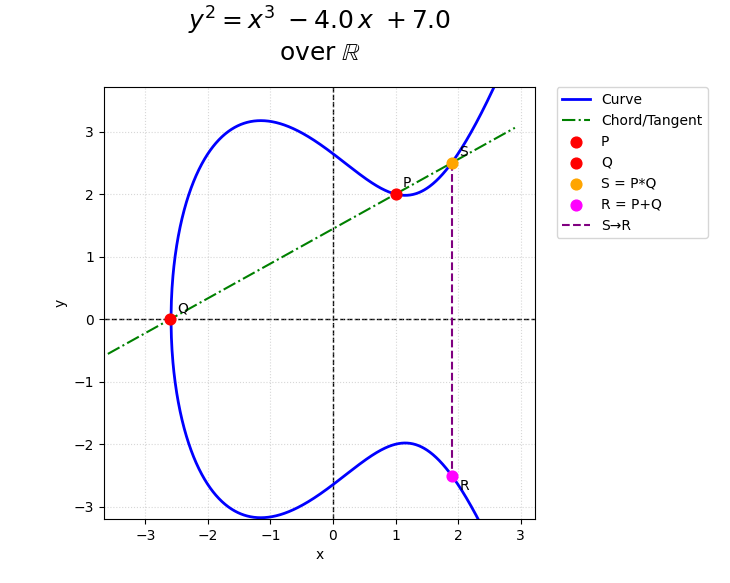
\includegraphics[width=\textwidth]{imagenes/elliptic_curve2D_addition_example.png}\\
    (a) Suma \(P+Q\)
  \end{minipage}\hfill
  \begin{minipage}{0.5\textwidth}
    \centering
    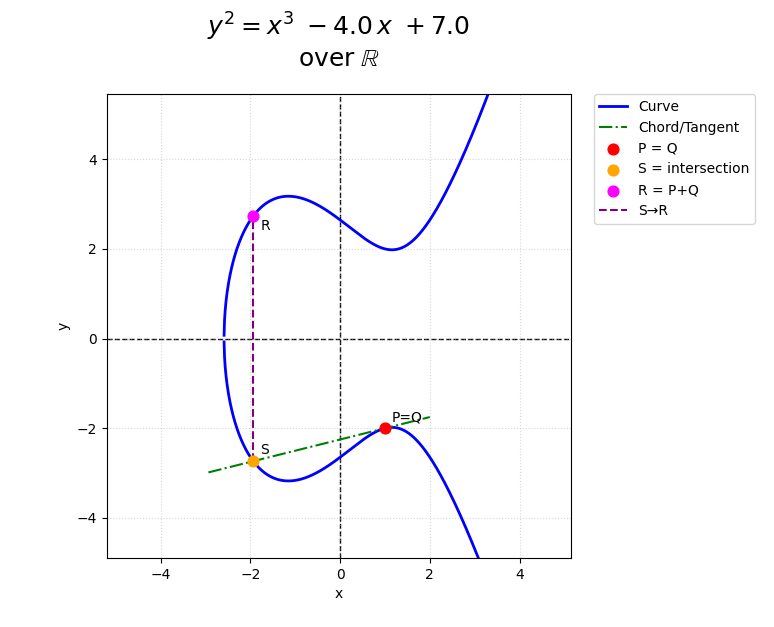
\includegraphics[width=\textwidth]{imagenes/elliptic_curve_same_addition_example.png}\\
    (b) Duplicación \(2P\)
  \end{minipage}
  \caption{Geometría de la ley de grupo en curvas elípticas}
  \label{fig:grupo_elipticas}
\end{figure}

\subsubsection*{Propiedades del grupo abeliano}
El conjunto de puntos de la curva, junto con la operación $+$ y el elemento neutro $\O$, forma un \emph{grupo abeliano} que denotamos
\[
  \bigl(E(K),\;+\,,\;\O\bigr).
\]
Este grupo verifica las siguientes propiedades:

\begin{enumerate}
  \item \textbf{Clausura.} Para todo $P,Q\in E(K)$, se tiene
    \[
      P + Q \;\in\; E(K).
    \]
  \item \textbf{Asociatividad.} Para todo $P,Q,R\in E(K)$,
    \[
      (P + Q) + R \;=\; P + (Q + R).
    \]
  \item \textbf{Elemento neutro.} Existe $\O\in E(K)$ tal que
    \[
      P + \O = \O + P = P,
      \quad \forall\,P\in E(K).
    \]
  \item \textbf{Inverso.} Para cada $P\in E(K)$ existe $-P\in E(K)$ (el opuesto de $P$)
    tal que
    \[
      P + (-P) = (-P) + P = \O.
    \]
  \item \textbf{Conmutatividad.} Para todo $P,Q\in E(K)$,
    \[
      P + Q = Q + P.
    \]
\end{enumerate}

\noindent En conjunto, estas cinco cláusulas definen un grupo abeliano (en particular, las cuatro primeras lo definen como grupo, y la quinta asegura que es abeliano).

\subsubsection*{Fórmulas en cuerpos de característica \(\neq2,3\)}

Para la forma corta de Weierstrass
\[
  E\colon\;y^2 = x^3 + a\,x + b,
  \quad a,b\in K,
  \quad \mathrm{char}(K)\neq2,3,
\]
las operaciones en coordenadas afines \((x,y)\) sobre \(K\) son:

\begin{enumerate}
  \item \emph{Negativo:} \(-P = (x,-y)\).
  \item \emph{Suma} \(P=(x_1,y_1)\), \(Q=(x_2,y_2)\), \(x_1\neq x_2\). Sea
    \[
      \lambda = \frac{y_2 - y_1}{x_2 - x_1}, 
      \quad
      x_3 = \lambda^2 - x_1 - x_2,\quad
      y_3 = \lambda(x_1 - x_3) - y_1.
    \]
    Entonces \(P + Q = (x_3,y_3)\).
  \item \emph{Duplicación} \(P=(x_1,y_1)\), \(y_1\neq0\). Sea
    \[
      \lambda = \frac{3x_1^2 + a}{2y_1}, 
      \quad
      x_3 = \lambda^2 - 2x_1,\quad
      y_3 = \lambda(x_1 - x_3) - y_1.
    \]
    Entonces \(2P = (x_3,y_3)\).
\end{enumerate}

\subsubsection*{Ley de grupo en campos binarios}

Cuando \(K = \F_{2^m}\) y la curva es no supersingular,
\[
  E\colon\;y^2 + x\,y = x^3 + A\,x^2 + B,
\]
la ley de grupo en \(\F_{2^m}\) (coordenadas afines) se implementa así:

\begin{enumerate}
  \item \emph{Negativo:} \(-P = (x,x+y)\).
  \item \emph{Suma} \(P=(x_1,y_1)\), \(Q=(x_2,y_2)\), \(x_1\neq x_2\). Sea
    \[
      \lambda = \frac{y_1 + y_2}{x_1 + x_2},\quad
      x_3 = \lambda^2 + \lambda + x_1 + x_2 + A,\quad
      y_3 = \lambda(x_1 + x_3) + x_3 + y_1.
    \]
    Entonces \(P + Q = (x_3,y_3)\).
  \item \emph{Duplicación} \(P=(x_1,y_1)\), \(x_1\neq0\). Sea
    \[
      \lambda = x_1 + \frac{y_1}{x_1},\quad
      x_3 = \lambda^2 + \lambda + A,\quad
      y_3 = x_1^2 + \lambda\,x_3 + x_3.
    \]
    Entonces \(2P = (x_3,y_3)\).
\end{enumerate}

Para curvas supersingulares en \(\F_{2^m}\) de la forma
\[
  E\colon\;y^2 + C\,y = x^3 + A\,x + B,
\]
las fórmulas cambian levemente (con \(-P=(x,y+C)\)), pero siguen el mismo patrón de suma y duplicación mediante \(\lambda\).



\subsection{Punto en el infinito}
\subsection{Ley de suma de puntos (geometría proyectiva)}

\section{Curvas sobre cuerpos finitos}\label{sec:curvas_sobre_cuerpos_finitos}
\begin{figure}[H]
    \centering
    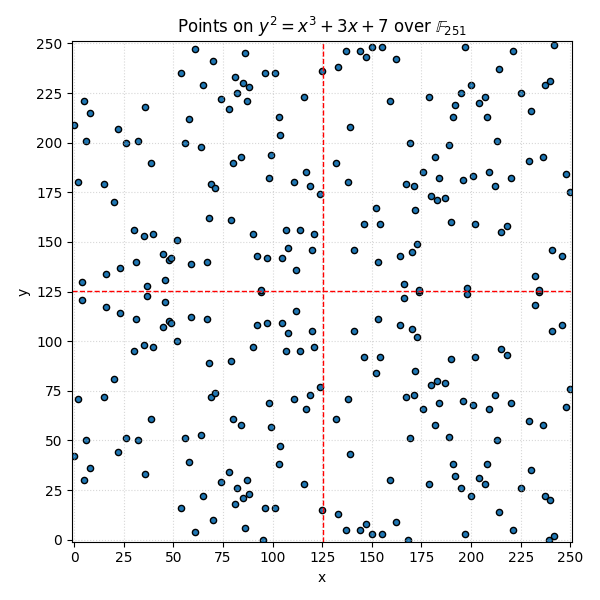
\includegraphics[width=0.8\textwidth]{imagenes/points_finite_field_251.png}
    \caption{Ejemplo de los puntos de una curva elíptica sobre un cuerpo finito}
    \label{fig:points_finite_field_251}
\end{figure}

\subsubsection*{Orden del grupo}

El número de puntos \(\#E(\F_q)\) se llama orden de la curva sobre \(\F_q\). Por el teorema de Hasse,
\[
  q + 1 - 2\sqrt{q} \;\le\;\#E(\F_q)\;\le\;q + 1 + 2\sqrt{q}.
\]
Este intervalo estrecho garantiza que \(\#E(\F_q)\approx q\), base de su resistencia criptográfica.
\subsection{Curvas sobre \texorpdfstring{$\mathbb{F}_p$}{Fp}}\label{sec:curvas_sobre_cuerpos_finitos_primos}
\subsection{Curvas binarias sobre \texorpdfstring{$\mathbb{F}_{2^m}$}{F2m}}\label{sec:curvas_sobre_cuerpos_finitos_binarios}

\section{Coordenadas y representación}\label{sec:coordenadas_curvas_elipticas}
\subsection{Coordenadas afines}
\subsection{Coordenadas proyectivas y Jacobianas}
\subsection{Coordenadas 'mixed' y optimizaciones}

\section{Selección de parámetros}
\subsection{Tamaños de curva y seguridad}
\subsection{Cofactores y subgrupos}
\subsection{Curvas estandarizadas (secp256k1, Curve25519, …)}
